\documentclass{article}

\usepackage{tabularx}
\usepackage{booktabs}
\usepackage{amsmath}
\usepackage{enumitem}
\usepackage{graphicx}
\usepackage{wrapfig}

\title{Usability Report\\\progname}

\author{\authname}

\date{}

\input{../Comments}
\input{../Common}

\begin{document}

\maketitle
\newpage

\section{Usability Testing Round 2}

\subsection{Overview of Goals}

In the context of our software, usability testing was conducted with the intention of mimicking the typical experience of a new user interacting with the software. The main goal of this testing was to understand how the user would intuitively engage with the software when given specific actionable prompts. We aim to collect data through direct user feedback and systematic observation of user interactions. The testing should also enable the integration of findings into the future development of our software. Ultimately, this is achieved through formalizing verbal feedback and observational insights into clearly defined requirements that will guide subsequent software updates.

\subsection{User Tasks}

The following section outlines the tasks that the users were asked to perform. The first 4 tasks should be complete in order. After the these four tasks have been completed, the user may interact with the software freely. There is no specifc order in which the final 7 actions have to be performed as long as all actions from 5 to 11 are completed by the end of usability testing. \\


\begin{description}[leftmargin=1.5cm, labelwidth=1.2cm, labelsep=0.5cm]

\item[\hypertarget{task:T1}{Task 1:}] Upload a new STL file.

\item[\hypertarget{task:T2}{Task 2:}] Open the STL file that was just uploaded.

\item[\hypertarget{task:T3}{Task 3:}] Create a new project to voxelize the STL model.

\item[\hypertarget{task:T4}{Task 4:}] Open the new voxelized project that you just created.

\item[\hypertarget{task:T5}{Task 5:}] Access the partition menu and use it to move to a different partition.

\item[\hypertarget{task:T6}{Task 6:}] Select a specific layer on the voxelized model.

\item[\hypertarget{task:T7}{Task 7:}] Move through different layers in the model.

\item[\hypertarget{task:T8}{Task 8:}] Select a group of at least six voxels at the same time.

\item[\hypertarget{task:T9}{Task 9:}] Assign a new material to a voxel.

\item[\hypertarget{task:T10}{Task 10:}] Assign a new magnetization value to a voxel.

\item[\hypertarget{task:T11}{Task 11:}] Export the CSV document for printing.

\end{description}

\newpage
\section{Participants}

These usability tests were conducted with our primary stakeholders. This consists of two grad students who were involved in developing the magnetic 3D printer and would be using this software to create their voxelized structures. The main graduate student who is continuing research for the 3D printer was the main participant who was testing the controls and attempting the specific actions from Section 2. The second graduate student requested to observe the session and provide relevant feedback based on the user’s interactions.

\section{Observations \& Feedback (Usability Test 1)}

This section summarizes all findings during each action. To ensure data integrity, testing was conducted mainly through observation to preserve a natural understanding of user-software interaction. When appropriate and necessary, prompting was provided when required, and direct information was obtained from discussion.

\subsection{Task 1}

\noindent The observations related to \hyperlink{task:T1}{Task 1} are as follows:\\

\noindent \hypertarget{finding:F311}{\textbf{Finding F311:}} 
The user spent a significant amount of time clicking the menu bar to try to figure out where this action is performed. In the end, they required prompting to figure out how to add a new STL file.\\ 

\noindent \textbf{Analysis \& Recommendations}: Per \hyperlink{finding:F331}{F311}, the significant time spent navigating the menu bar may be partly due to the user exploring unfamiliar software, but it also suggests that certain elements of the interface may be unintuitive and not easily discoverable. There should be consideration towards adding the following requirement to support initial user interaction:

\begin{center}
  \textit{The system shall provide an initial screen that opens upon launching the application to assist users in beginning the application workflow.}
\end{center}


\subsection{Task 2}

\noindent The observations related to \hyperlink{task:T2}{Task 2} are as follows:\\

\noindent \hypertarget{finding:F321}{\textbf{Finding F321:}} 
There is natural confusion on why the user had to upload a new STL file and then perform a separate action in order for the STL file to actually load. While this action was included in the list of attempted actions, the user had to be prompted to do the action again. \\ 

\noindent \textbf{Analysis \& Recommendations}:
Per \hyperlink{finding:F321}{F321}, the workflow is unintuitive and the code should have different workflow operations for opening a previously uploaded STL file versus uploading a new STL file. There should be consideration towards adding the following requirement:

\begin{center}
  \textit{The system shall open the STL file automatically }\\
  \textit{when a new STL file is uploaded.}
\end{center}

\subsection{Task 3}

\noindent The observations related to \hyperlink{task:T3}{Task 3} are as follows:\\

\noindent \hypertarget{finding:F331}{\textbf{Finding F331:}} 
The user had to ask for clarification on how the model and voxel scaling worked.  \\ 

\noindent \hypertarget{finding:F332}{\textbf{Finding F332:}} 
The user had difficulty choosing a proper voxel size to be applied to the model. \\ 

\noindent \hypertarget{finding:F333}{\textbf{Finding F333:}} 
If a new name is not chosen, then two structures are made under the same file name. \\ 


\noindent \textbf{Analysis \& Recommendations}:
Per \hyperlink{finding:F331}{F331}, model scaling should be adjusted to better fit typical structure units. There should be consideration towards changing the selection of measurements to the following options: micrometres, millimetres, and centimetres.\\

\noindent Per \hyperlink{finding:F332}{F332}, there is a lack of intuitive understanding on how the model will be voxelized when inputting a specific voxel measurement. There should be consideration towards adding the following requirement to facilitate user understanding on how many voxels will be created during project creation based on the voxel size that is input:

\begin{center}
  \textit{The system shall provide STL model measurements during project creation.}\\
\end{center}

\noindent Per \hyperlink{finding:F333}{F333}, there is no warning, overriding of the old project, or explicit prevention of two files being created with the same name. This leads to two structures existing in the same SQL database. There should be consideration towards adding the following constraint:

\begin{center}
  \textit{The system shall validate project names before creation to ensure that no duplicate file names are used. }\\
\end{center}


\subsection{Task 4}

\noindent The observations related to \hyperlink{task:T4}{Task 4} are as follows:\\

\noindent \hypertarget{finding:F341}{\textbf{Finding F341:}} 
The user assumed that after creating a new project, it would automatically open.\\ 

\noindent \textbf{Analysis \& Recommendations}:
Per \hyperlink{finding:F341}{F341}, access to a new project does not following intuitive logic. There should be consideration towards adding the following requirement:

\begin{center}
  \textit{The system shall open a project automatically upon creation. }\\
\end{center}

\subsection{Task 5}

\noindent The observations related to \hyperlink{task:T5}{Task 5} are as follows:\\

\noindent \hypertarget{finding:F351}{\textbf{Finding F351:}} 
The user had difficulty understanding how the partitions related to each other, especially since all partitions were centered in the middle.\\ 

\noindent \hypertarget{finding:F352}{\textbf{Finding F352:}} 
The user noted that if partitions looked similar, there was no way to determine which part of the model each partition corresponded to.\\ 

\noindent \hypertarget{finding:F353}{\textbf{Finding F353:}} 
The user expressed a desire for the ability to rename partitions in the sidebar, as it would allow them to create personalized labels that match their own interpretation of the partitions.\\ 

\noindent \hypertarget{finding:F354}{\textbf{Finding F354:}} 
The user noted that allowing the partition size to be selected could be beneficial, though it is considered a nice-to-have rather than a necessity. \\ 

\noindent \textbf{Analysis \& Recommendations}:
Per \hyperlink{finding:F351}{F351} \& \hyperlink{finding:F352}{F352}, the current partition system in unintuitive to navigate through. There should be consideration towards additing the following requirement:

\begin{center}
  \textit{The system shall present sufficient information in the partition bar to enable users to understand how each partition fits within the model without needing to select it.}\\
\end{center}

\noindent If possible, options should be explored to provide a visualization aspect to the partition bar, as that would likely provide the best intuitive understanding of how the partitions fit within the model.\\

\noindent Per \hyperlink{finding:F353}{F353}, allowing the user to rename a partition may also help ease the process of understanding how partitions relate to one another. There should be consideration towards adding the following requirement:

\begin{center}
    \textit{The system shall allow the user to rename a partition in the partition sidebar, enabling personalized interpretation of the model’s structure.}\\
  \end{center}

  \noindent Per \hyperlink{finding:F354}{F354}, there should be consideration towards allowing the user to select their desired partition size during initial project creation. While not a current necessity, in future development, it may become a requirement to enhance the system.


  \subsection{Task 6}

\noindent The observations related to \hyperlink{task:T6}{Task 6} are as follows:\\

\noindent \hypertarget{finding:F361}{\textbf{Finding F361:}} 
The user was able to easily select a layer on the voxelized model.\\ 

\noindent \textbf{Analysis \& Recommendations}: Due to the ease of performing this action for the user, no significant system changes are required to support user interaction in this regard.

\subsection{Task 7}

\noindent The observations related to \hyperlink{task:T7}{Task 7} are as follows:\\

\noindent \hypertarget{finding:F371}{\textbf{Finding F371:}} 
The user moved through the layers by manually select a different layer.\\ 

\noindent \hypertarget{finding:F372}{\textbf{Finding F372:}} 
The user also noted that arranging the layers horizontally (see Figure 1), with navigation occurring up and down, would feel more intuitive, as it better aligns with how the model is printed.\\ 

\noindent \textbf{Analysis \& Recommendations}:
Per \hyperlink{finding:F371}{F371}, it seemed that their first instinct was to just manually select a different layer rather than use the up and down arrow buttons on the side of the layer viewer. This raises the question of whether the arrows for navigating layers are sufficiently visible and intuitive compared to directly selecting a layer. However, considering that users tend to rely on familiar interactions—and that manual selection is typically their initial method of engaging with the layer editor—it is reasonable to conclude that, regardless of how the arrows are presented, users will naturally default to manually selecting layers if they are unaware of alternative features. This means that it is important to clearly document the arrow controls in the user manual to raise awareness of this functionality.\\

\begin{wrapfigure}{r}{0.20\textwidth} 
    \centering
    \fbox{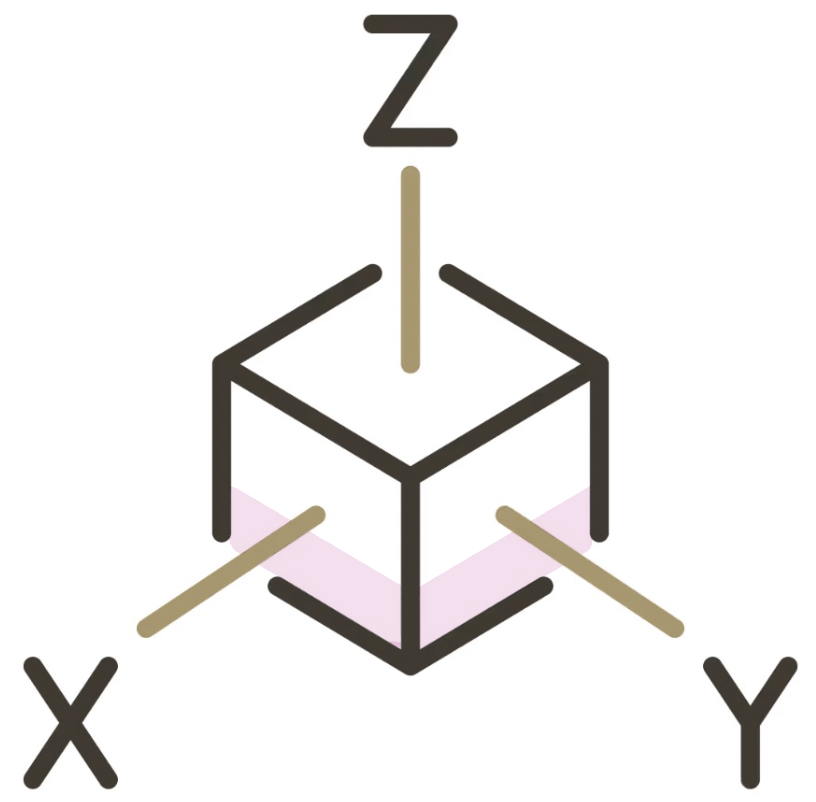
\includegraphics[width=0.20\textwidth]{Figure1.png}}
    \caption{Model axis diagram}
\end{wrapfigure}

\noindent Per \hyperlink{finding:F372}{F372}, users were able to move through the layers with ease. However, natural intuitiveness is important within software. Therefore, aligning the structure with what the user typically visualizes during the printing process is important for high-quality user interaction. 

\noindent Consider making the requirement for layer slicing more explicit. For example:

\begin{center}
    \textit{The system shall implement layer slicing horizontally along the z-axis, assuming axes conform to how they are expressed in Figure 1. }\\
\end{center}


\subsection{Task 8}

\noindent The observations related to \hyperlink{task:T8}{Task 8} are as follows:\\

\noindent \hypertarget{finding:F381}{\textbf{Finding F381:}} 
The user initially required a moment to understand how to select multiple voxels at once. However, once familiar with it, the user explicitly stated that they appreciated the feature, as it enabled efficient selection of irregularly shaped voxel groups.\\ 

\noindent \textbf{Analysis \& Recommendations}:
Per \hyperlink{finding:F381}{F381}, the extra time taken to figure out how to use the lasso feature is likely because the lasso feature is typically not the most conventional method for group selection. However, since the user responded positively to the method of group selection, no significant system changes are required. Any confusion arising from the unconventional method of group selection seems to be minor and can be addressed through the user manual. 

\subsection{Task 9}

\noindent The observations related to \hyperlink{task:T9}{Task 9} are as follows:\\

\noindent \hypertarget{finding:F391}{\textbf{Finding F391:}} 
The user was able to intuitively navigate the process of assigning a new material to both an individual voxel and a group of voxels at the same time.\\ 

\noindent \textbf{Analysis \& Recommendations}:
Due to the ease of performing this action for the user, no significant system changes are required to support user interaction in this regard.

\subsection{Task 10}

\noindent The observations related to \hyperlink{task:T10}{Task 10} are as follows:\\

\noindent \hypertarget{finding:F3101}{\textbf{Finding F3101:}} 
When assigning a magnetization, the user stated that adding magnitude metadata is unnecessary, as it is not required by the 3D printer.\\ 

\noindent \hypertarget{finding:F3101}{\textbf{Finding F3102:}} 
The user also expressed a desire for there to be a way to easily check which voxels have been assigned a magnetized value without having to go through each voxel.\\ 

\noindent \textbf{Analysis \& Recommendations}:
Per \hyperlink{finding:F3101}{F3101}, the system should be adjusted to only require angles for magnetization metadata.\\

\noindent Per \hyperlink{finding:F3102}{F3102}, this is a failure to implement a requirement that already exists. Current requirement documentation states the following:

\begin{center}
    \textit{Visualization Manager shall integrate easy tracking of voxels that have been assigned magnetization vectors by providing the option to toggle the colour of all magnetized voxels. }\\
  \end{center}

This requirement should now be prioritized for implementation. However, the method of showing which voxels are magnetized may change.

\subsection{Task 11}

\noindent The observations related to \hyperlink{task:T11}{Task 11} are as follows:\\

\noindent \hypertarget{finding:F3111}{\textbf{Finding F3111:}} 
The user was able to easily export the CSV document for printing. When looking at the CSV document exported, there were no suggested changes to the information that was contained within the CSV document or the format within the CSV file.\\ 

\noindent \textbf{Analysis \& Recommendations}:
Due to the ease of performing this action for the user, no significant system changes are required to support user interaction in this regard.

\section{Results from User Survey}

This survey occurs at the end of the first usability test. 


\subsection{Survey Questions}

The following section presents the survey questions, each evaluated using a 5-point scale. The meanings of both endpoints of the scale are provided below.

\begin{description}[leftmargin=2.5cm, labelwidth=1.2cm, labelsep=0.5cm]

    \item[\hypertarget{question:T1}{Question 1:}] How difficult was it for you to navigate the overall interface?
    \item[] \hspace{0.7cm} \textit{Rating Scale:} 1 = very easy, 5 = high difficulty 
    \item[\hypertarget{question:T2}{Question 2:}] Do you consider the current method of moving the model to inspect it intuitive?
    \item[] \hspace{0.7cm} \textit{Rating Scale:} 1 = not intuitive, 5 = highly intuitive 
    \item[\hypertarget{question:T3}{Question 3:}] How natural do you find the layer select functionality?
    \item[] \hspace{0.7cm} \textit{Rating Scale:} 1 = not natural, 5 = very natural 
    \item[\hypertarget{question:T4}{Question 4:}]  How intuitive did you find the method of selecting voxels?
    \item[] \hspace{0.7cm} \textit{Rating Scale:} 1 = not intuitive, 5 = highly intuitive 
    \item[\hypertarget{question:T5}{Question 5:}] How easy was it for you to assign a magnetization to a set of voxels?
    \item[] \hspace{0.7cm} \textit{Rating Scale:} 1 = very difficult, 5 = very easy 
    \item[\hypertarget{question:T6}{Question 6:}] How easy was it for you to assign a material to a set of voxels?
    \item[] \hspace{0.7cm} \textit{Rating Scale:} 1 = very difficult, 5 = very easy 
    \item[\hypertarget{question:T7}{Question 7:}] Do you find the current signifiers for completed voxels helpful?
    \item[] \hspace{0.7cm} \textit{Rating Scale:} 1 = not helpful, 5 = very helpful 
    \item[\hypertarget{question:T8}{Question 8:}] How intuitive did you find the file importing process?
    \item[] \hspace{0.7cm} \textit{Rating Scale:} 1 = not intuitive, 5 = highly intuitive  
    \item[\hypertarget{question:T9}{Question 9:}] How intuitive did you find the file exporting process?
    \item[] \hspace{0.7cm} \textit{Rating Scale:} 1 = not intuitive, 5 = highly intuitive 

\end{description}

\subsection{Survey Results}

The following section provides the user results as well as outlines how any additional comments the user felt relevant to include in relation to the question.

\begin{figure}[h]
    \centering
    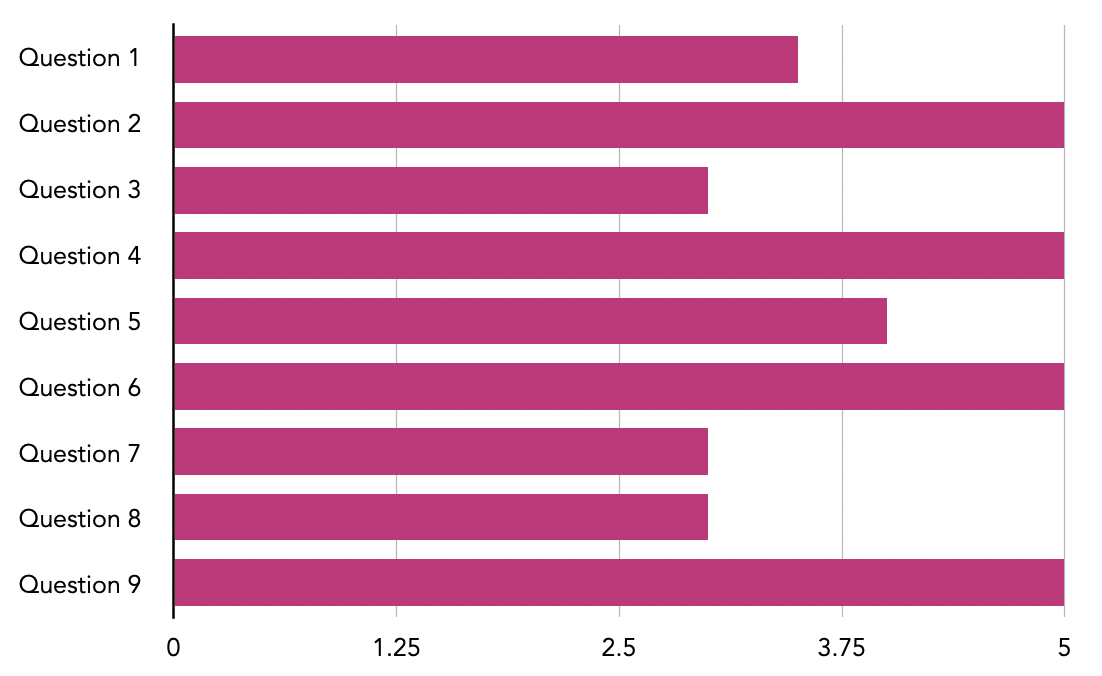
\includegraphics[width=0.8\textwidth]{Figure2.png}
    \caption{Summary of Usability Survey Results}
    \label{fig:survey-results}
\end{figure}



\section{Observations \& Feedback (Usability Test 2)}

These usability tests were conducted with only the primary grad students who created the magnetic 3D printer present. The following section replicates the actions performed in Section 2 after addressing issues identified through the findings in Section 3. To ensure data integrity, testing was conducted mainly through observation to preserve a natural understanding of user-software interaction. When appropriate and necessary, prompting was provided when required, and direct information was obtained from discussion.

\noindent This section includes only new observations identified during this round of usability testing. Any previously documented observations from the initial round that remain unimplemented have been excluded.

\subsection{Tasks 1 Through 4}

\noindent The observations related to \hyperlink{task:T1}{Task 1}, \hyperlink{task:T2}{Task 2}, \hyperlink{task:T3}{Task 3} \& \hyperlink{task:T4}{Task 4} are as follows:\\

\noindent \textbf{Feedback on Implemented Changes from First Usability Test:}: In the second iteration of usability testing, these actions were grouped together due to the introduction of a new workflow. This workflow provides a more intuitive progression through the steps required to create a new project or access an existing one, making it appropriate to assess these actions as a whole. Observations showed that users were able to complete these actions more smoothly, with noticeably less confusion, as the system more effectively guided them through the process rather than requiring them to search for how to proceed. Additionally, the user asked fewer questions, further supporting the conclusion that the revised workflow enhanced usability and overall user experience during the entire process of creating a project.\\

\noindent \hypertarget{finding:F511}{\textbf{Finding F511:}} N/A\\

\noindent There remain no notable issues for the user while performing these actions. No significant system changes in relation to this interaction were identified from this round of usability testing.

\subsection{Task 5}

\noindent The observations related to \hyperlink{task:T5}{Task 5} are as follows:\\

\noindent \textbf{Feedback on Implemented Changes from First Usability Test:}: A visual 3D map was added within the partition menu to show how the partitions relate to each other. When a partition is selected, it shows where that partition maps within the model. This was a change implemented to address \hyperlink{finding:F351}{F351} and \hyperlink{finding:F352}{F352}. The overall response from the user was positive, and they said that they were satisfied with the improvement. Both through observed interaction and direct user feedback, it was evident that the added visualization clarified the spatial relationships between partitions and made them significantly easier to understand.\\

\noindent The user also appreciated that they were able to rename the partitions. This was a change implemented due to \hyperlink{finding:F353}.

\noindent \hypertarget{finding:F521}{\textbf{Finding F521:}} 
While switching through the partitions, the user had to repeatedly adjust the model view, as the partition sidebar partially obstructed the structure when it was open. This caused minor annoyance, and the user expressed a preference for preserving any changes to the viewpoint when navigating between partitions.\\ 

\noindent \textbf{Analysis \& Recommendations}:
Per \hyperlink{finding:F521}{F521}, the underlying issue appears to stem from the model being frequently obstructed by the partition sidebar. Consideration should be given to preserving the user’s viewpoint during partition navigation, as suggested by the user. Alternatively, dynamically adjusting the model’s position when the partition menu is opened or closed may also help mitigate this issue.

\subsection{Tasks 6}

\noindent There remain no notable issues for the user while performing these actions. No significant system changes in relation to this interaction were identified from this round of usability testing.

\subsection{Task 7}

\noindent The observations related to \hyperlink{task:T7}{Task 7} are as follows:\\

\noindent \textbf{Feedback on Implemented Changes from First Usability Test:}: When selecting a layer, the user confirmed that the slicing orientation and the up/down navigation between layers aligned with how they typically visualize the model in relation to the printing process. This was a change implemented due to finding \hyperlink{finding:F372}{F372}.\\

\noindent \hypertarget{finding:F541}{\textbf{Finding F541:}} N/A

\noindent There remain no notable issues for the user while performing these actions. No significant system changes in relation to this interaction were identified from this round of usability testing.

\subsection{Task 8}

\noindent The observations related to \hyperlink{task:T8}{Task 8} are as follows:\\

\noindent \hypertarget{finding:F551}{\textbf{Finding F551:}} 
The user naturally attempted to select a rectangular group of voxels by clicking and holding at one corner of the desired region and dragging to the opposite corner to define the selection area. It was suggested that incorporating this conventional method of group selection would improve usability. \\

\noindent \hypertarget{finding:F552}{\textbf{Finding F552:}} 
The user also specifically indicated a preference for an additional option, beyond the lasso tool, that allows multiple non-contiguous voxels to be selected by holding a key (e.g., Shift) and selecting voxels across different areas of the structure, even when those regions are not connected.\\ 

\noindent \textbf{Analysis \& Recommendations}:
Per \hyperlink{finding:F551}{F551}, to improve user experience, it may be ideal to incorporate both conventional methods of group selection (e.g., hold and drag) in addition to the slightly more unconventional method (e.g., lasso) to provide users with more freedom in group voxel selection.\\

\noindent Per \hyperlink{finding:F552}{F552}, there should be consideration towards adding the following requirement:

\begin{center}
    \textit{The system shall allow multiple non-contiguous voxels}\\
    \textit{to be selected within the same group voxel selection.}
  \end{center}
  
\subsection{Task 9}

\noindent The observations related to \hyperlink{task:T9}{Task 9} are as follows:\\

\noindent \hypertarget{finding:F561}{\textbf{Finding F561:}} 
After saving a material, the user indicated a preference for the bottom panel—used to set magnetization and material values in the layer viewer—to remain visible at all times, rather than appearing only after a voxel selection is made. \\

\noindent \textbf{Analysis \& Recommendations}:
Per \hyperlink{finding:F561}{F561}, it is a reasonable desire to want the interface to always remain visible, as it supports intuitive interaction by clearly indicating where users can modify metadata when accessing the layer editor. However, if this is implemented, there should be consideration towards adding the following constraint: 

\begin{center}
    \textit{The system shall ensure no metadata is able to be changed }\\
    \textit{unless there is an active selection of voxels.}
\end{center}

\noindent Note that the above recommended action is also relevant to consider for \hyperlink{task:T10}{Task 10}.


\subsection{Task 10}

\noindent The observations related to \hyperlink{task:T10}{Task 10} are as follows:\\

\noindent \textbf{Feedback on Implemented Changes from First Usability Test:} Upon saving the magnetization, the user was pleased with the checkmarks that indicate that the voxel was assigned a magnetization. This was a change implemented due to \hyperlink{finding:F3102}{F3102}.\\

\noindent \hypertarget{finding:F571}{\textbf{Finding F571:}} 
After entering values into the magnetization input fields, the user instinctively pressed Enter to save the changes. When asked directly, the user indicated that implementing this shortcut would be a helpful addition alongside the existing button for saving magnetization. \\

\noindent \textbf{Analysis \& Recommendations}:
Per \hyperlink{finding:F571}{F571}, implementing a keyboard shortcut using Enter to update magnetization values after input would be ideal, as it aligns with common user expectations and standard interaction patterns.

\subsection{Tasks 11}

\noindent There remain no notable issues for the user while performing these actions. No significant system changes in relation to this interaction were identified from this round of usability testing.
  
\end{document}